% Options for packages loaded elsewhere
\PassOptionsToPackage{unicode}{hyperref}
\PassOptionsToPackage{hyphens}{url}
%
\documentclass[
]{article}
\usepackage{amsmath,amssymb}
\usepackage{lmodern}
\usepackage{iftex}
\ifPDFTeX
  \usepackage[T1]{fontenc}
  \usepackage[utf8]{inputenc}
  \usepackage{textcomp} % provide euro and other symbols
\else % if luatex or xetex
  \usepackage{unicode-math}
  \defaultfontfeatures{Scale=MatchLowercase}
  \defaultfontfeatures[\rmfamily]{Ligatures=TeX,Scale=1}
\fi
% Use upquote if available, for straight quotes in verbatim environments
\IfFileExists{upquote.sty}{\usepackage{upquote}}{}
\IfFileExists{microtype.sty}{% use microtype if available
  \usepackage[]{microtype}
  \UseMicrotypeSet[protrusion]{basicmath} % disable protrusion for tt fonts
}{}
\makeatletter
\@ifundefined{KOMAClassName}{% if non-KOMA class
  \IfFileExists{parskip.sty}{%
    \usepackage{parskip}
  }{% else
    \setlength{\parindent}{0pt}
    \setlength{\parskip}{6pt plus 2pt minus 1pt}}
}{% if KOMA class
  \KOMAoptions{parskip=half}}
\makeatother
\usepackage{xcolor}
\usepackage[margin=1in]{geometry}
\usepackage{graphicx}
\makeatletter
\def\maxwidth{\ifdim\Gin@nat@width>\linewidth\linewidth\else\Gin@nat@width\fi}
\def\maxheight{\ifdim\Gin@nat@height>\textheight\textheight\else\Gin@nat@height\fi}
\makeatother
% Scale images if necessary, so that they will not overflow the page
% margins by default, and it is still possible to overwrite the defaults
% using explicit options in \includegraphics[width, height, ...]{}
\setkeys{Gin}{width=\maxwidth,height=\maxheight,keepaspectratio}
% Set default figure placement to htbp
\makeatletter
\def\fps@figure{htbp}
\makeatother
\setlength{\emergencystretch}{3em} % prevent overfull lines
\providecommand{\tightlist}{%
  \setlength{\itemsep}{0pt}\setlength{\parskip}{0pt}}
\setcounter{secnumdepth}{-\maxdimen} % remove section numbering
\usepackage{booktabs}
\usepackage{longtable}
\usepackage{array}
\usepackage{multirow}
\usepackage{wrapfig}
\usepackage{float}
\usepackage{colortbl}
\usepackage{pdflscape}
\usepackage{tabu}
\usepackage{threeparttable}
\usepackage{threeparttablex}
\usepackage[normalem]{ulem}
\usepackage{makecell}
\usepackage{xcolor}
\ifLuaTeX
  \usepackage{selnolig}  % disable illegal ligatures
\fi
\IfFileExists{bookmark.sty}{\usepackage{bookmark}}{\usepackage{hyperref}}
\IfFileExists{xurl.sty}{\usepackage{xurl}}{} % add URL line breaks if available
\urlstyle{same} % disable monospaced font for URLs
\hypersetup{
  pdftitle={Supplementary Materials WEIRD CHILDES},
  pdfauthor={Camila Scaff},
  hidelinks,
  pdfcreator={LaTeX via pandoc}}

\title{Supplementary Materials WEIRD CHILDES}
\author{Camila Scaff}
\date{2024-02-26}

\begin{document}
\maketitle

\hypertarget{sm1-partial-correlations-of-the-four-dimensions-of-interest}{%
\subsection{SM1 :Partial correlations of the four dimensions of
interest}\label{sm1-partial-correlations-of-the-four-dimensions-of-interest}}

\begin{figure}
\centering
\includegraphics{Supplementary_analyses_WEIRDCHILDES_files/figure-latex/scatterplot matrix-1.pdf}
\caption{Evidence of partial correlations of the four continous
dimensions of interest. The diagonal shows density of the distribution
of each of the variables. Panels below the diagonal show the scatter
plot for the two variables involved (e.g., proportion completed
highschool and percentage urban for the second row, first column). Those
above the diagonal show the Pearson correlation for the two variables
involved. Education is represented by proportion of the population
completing lower secondary school; industrialization by proportion of
the population living in urban (as opposed to rural) sites; richness by
GDP per capita.}
\end{figure}

\hypertarget{sm2-flowchart}{%
\subsection{SM2 Flowchart}\label{sm2-flowchart}}

\begin{figure}
\centering
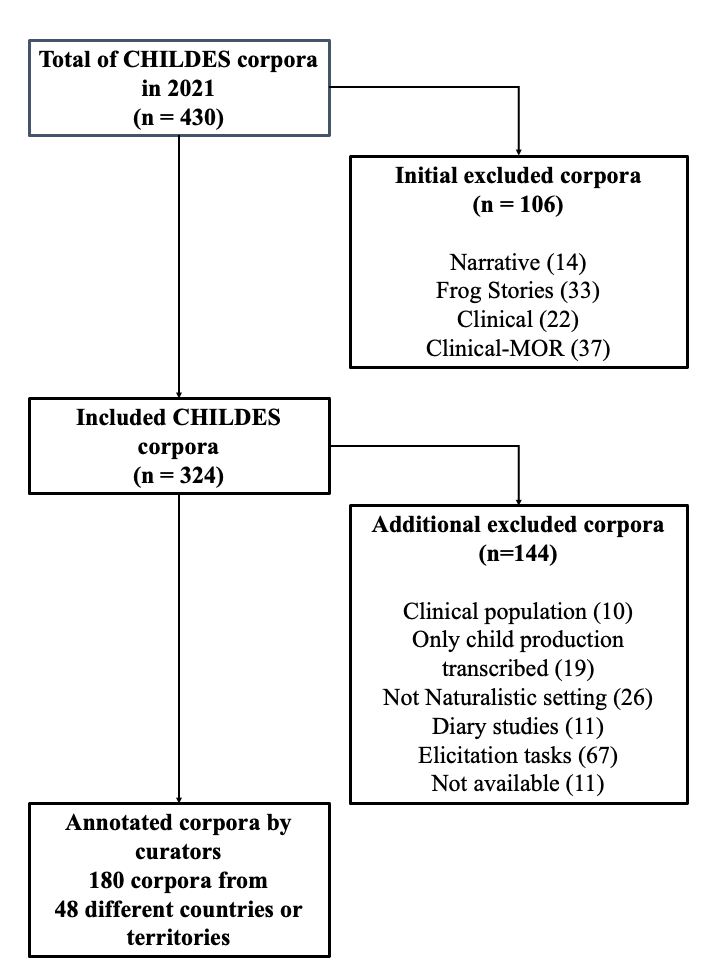
\includegraphics{../figures/flowchart.png}
\caption{Flowchart}
\end{figure}

\hypertarget{sm3-sources-used-for-density-plot}{%
\subsection{SM3: Sources used for Density
plot}\label{sm3-sources-used-for-density-plot}}

The goal of the country-level analysis is to assess the
representativeness of our sub-sample of CHILDES against world
statistics. For this, we first identified the country where the
recordings were collected. The following variables were used for this
level of analysis, all derived from official sources including the World
Bank, Our World in Data (WDI), and the United Nations (UN). For each
macro-dimension described in the Introduction, we looked for relevant
world statistics available (see the annotated code for more details
about the indicators). SES For the SES dimension we choose two measures
representing education and income. For the education measure, we turned
to Our World in Data (WDI), an organization that collates information
from various official sources. We downloaded information on the
proportion of the population that had completed lower secondary school
(data from 2007-2015; Our World in Data, 2022a; see Supplementary
Materials (SMX) for figures using the proportion of the population
completing high school instead). For the income measure, we relied on
the World Development Indicators (WDI) from the World Bank, available
via the WDI package in R (Vincent Arel-Bundock, 2021). We choose the
Gross Domestic Product (GDP) per capita (based on log 10), a measure
that represents how relatively rich countries are based on 2017 US
dollars purchasing power parity. It is expressed in 2017 US dollars.

Urbanization We used the percentage of the population living in urban
areas indicator, from the WDI from the World Bank. It represents the
proportion of the population that was rural, so we estimated the
complement to 100\% to conceptually align this variable to the others.
We employed indicators for the year 2011 because this was the year in
which we had the maximum amount of data available for those variables.
Family structure We used two measures pertaining to household size from
the UN database on Household Size and Composition 2022 (data from
2000-2022 United Nations, 2022). First, the average number of household
members, and second, the average number of members under the age of 15.

\begin{center}
\begin{ThreePartTable}

\begin{longtable}{lcc}\noalign{\getlongtablewidth\global\LTcapwidth=\longtablewidth}
\caption{\label{tab:tab1}}\\
\toprule
Dimension & \multicolumn{1}{c}{Macro.level.variable} & \multicolumn{1}{c}{Source}\\
\midrule
\endfirsthead
\caption*{\normalfont{Table \ref{tab:tab1} continued}}\\
\toprule
Dimension & \multicolumn{1}{c}{Macro.level.variable} & \multicolumn{1}{c}{Source}\\
\midrule
\endhead
SES & Percent of the population completing lower secondary school* & Data from 2007-2015; Our World in Data, 2022a\\
SES & GDP per capita (log 10) & World Development Indicators (WDI) from the World Bank, available via the WDI package in R (Vincent Arel-Bundock, 2021)\\
Urbanization & Percent of the population living in urban areas & WDI from the World Bank. It represents the proportion of the population that was rural, so we estimated the complement to 100\% to conceptually align this variable to the others. We employed indicators for the year 2011 because this was the year in which we had the maximum amount of data available for those variables.\\
Family structure & Average household size & UN database on Household Size and Composition 2022 (data from 2000-2022 United Nations, 2022)\\
Family structure & Average number of member under 15 in households & UN database on Household Size and Composition 2022 (data from 2000-2022 United Nations, 2022)\\
Language & NA & NA\\
\bottomrule
\end{longtable}

\end{ThreePartTable}
\end{center}

\hypertarget{sm4-distribution-of-childes-participants-by-country-and-continent}{%
\subsection{SM4: Distribution of CHILDES participants by country and
continent}\label{sm4-distribution-of-childes-participants-by-country-and-continent}}

\begin{center}
\begin{ThreePartTable}

\begin{longtable}{lcc}\noalign{\getlongtablewidth\global\LTcapwidth=\longtablewidth}
\caption{\label{tab:tab2}Descriptives}\\
\toprule
country & \multicolumn{1}{c}{TimesRepeated} & \multicolumn{1}{c}{TotalParticipants\_country}\\
\midrule
\endfirsthead
\caption*{\normalfont{Table \ref{tab:tab2} continued}}\\
\toprule
country & \multicolumn{1}{c}{TimesRepeated} & \multicolumn{1}{c}{TotalParticipants\_country}\\
\midrule
\endhead
Argentina & 1 & 1\\
Austria & 1 & 1\\
Belgium & 4 & 40\\
Brazil & 1 & 1\\
Canada & 3 & 8\\
China & 7 & 174\\
Croatia & 1 & 3\\
Czech Republic & 1 & 6\\
Denmark & 2 & 3\\
Egypt & 1 & 10\\
Estonia & 8 & 32\\
France & 11 & 51\\
Germany & 7 & 55\\
Greece & 2 & 6\\
Hong Kong & 2 & 8\\
Hungary & 4 & 10\\
Iceland & 1 & 1\\
India & 1 & 1\\
Indonesia & 1 & 8\\
Iran & 2 & 5\\
Ireland & 2 & 7\\
Israel & 7 & 123\\
Italy & 5 & 10\\
Jamaica & 1 & 2\\
Japan & 6 & 140\\
Kuwait & 1 & 70\\
Lesotho & 1 & 4\\
Mexico & 2 & 2\\
Netherlands & 6 & 22\\
Norway & 2 & 11\\
Papua New Guinea & 1 & 5\\
Poland & 1 & 4\\
Portugal & 2 & 8\\
Romania & 2 & 6\\
Russia & 1 & 1\\
Serbia & 1 & 8\\
Singapore & 1 & 55\\
Slovenia & 1 & 20\\
South Africa & 1 & 2\\
South Korea & 2 & 4\\
Spain & 23 & 211\\
Spain \& Hungary & 1 & 1\\
Sweden & 3 & 9\\
Sweden \& Portugal & 1 & 3\\
Switzerland & 1 & 1\\
Taiwan & 1 & 4\\
Thailand & 1 & 18\\
Turkey & 1 & 1\\
United Kingdom & 11 & 560\\
United States & 30 & 405\\
\bottomrule
\end{longtable}

\end{ThreePartTable}
\end{center}

\begin{center}
\begin{ThreePartTable}

\begin{longtable}{lcc}\noalign{\getlongtablewidth\global\LTcapwidth=\longtablewidth}
\caption{\label{tab:tab3}Descriptives}\\
\toprule
region & \multicolumn{1}{c}{TimesRepeated} & \multicolumn{1}{c}{TotalParticipants\_continent}\\
\midrule
\endfirsthead
\caption*{\normalfont{Table \ref{tab:tab3} continued}}\\
\toprule
region & \multicolumn{1}{c}{TimesRepeated} & \multicolumn{1}{c}{TotalParticipants\_continent}\\
\midrule
\endhead
Africa & 3 & 16\\
Americas & 38 & 419\\
Asia & 33 & 611\\
Europe & 105 & 1090\\
Oceania & 1 & 5\\
\bottomrule
\end{longtable}

\end{ThreePartTable}
\end{center}

\hypertarget{sm5-table-of-urban-indicators-by-country-using-most-recent-date-available-2022}{%
\subsection{SM5: Table of urban indicators by country, using most recent
date available
(2022)}\label{sm5-table-of-urban-indicators-by-country-using-most-recent-date-available-2022}}

This indicator is based in the World Bank staff estimates based on the
United Nations Population Division's World Urbanization Prospects: 2018
Revision.

\begin{center}
\begin{ThreePartTable}

\begin{longtable}{lc}\noalign{\getlongtablewidth\global\LTcapwidth=\longtablewidth}
\caption{\label{tab:tab4}Urban indicator by country included in CHILDES sample}\\
\toprule
Country & \multicolumn{1}{c}{\% Urban}\\
\midrule
\endfirsthead
\caption*{\normalfont{Table \ref{tab:tab4} continued}}\\
\toprule
Country & \multicolumn{1}{c}{\% Urban}\\
\midrule
\endhead
Argentina & 92.35\\
Austria & 59.26\\
Belgium & 98.15\\
Belgium & 98.15\\
Belgium & 98.15\\
Belgium & 98.15\\
Brazil & 87.56\\
Canada & 81.75\\
Canada & 81.75\\
Canada & 81.75\\
Switzerland & 74.09\\
China & 63.56\\
China & 63.56\\
China & 63.56\\
China & 63.56\\
China & 63.56\\
China & 63.56\\
China & 63.56\\
Czechia & 74.38\\
Germany & 77.65\\
Germany & 77.65\\
Germany & 77.65\\
Germany & 77.65\\
Germany & 77.65\\
Germany & 77.65\\
Germany & 77.65\\
Denmark & 88.37\\
Denmark & 88.37\\
Egypt, Arab Rep. & 42.97\\
Spain & 81.30\\
Spain & 81.30\\
Spain & 81.30\\
Spain & 81.30\\
Spain & 81.30\\
Spain & 81.30\\
Spain & 81.30\\
Spain & 81.30\\
Spain & 81.30\\
Spain & 81.30\\
Spain & 81.30\\
Spain & 81.30\\
Spain & 81.30\\
Spain & 81.30\\
Spain & 81.30\\
Spain & 81.30\\
Spain & 81.30\\
Spain & 81.30\\
Spain & 81.30\\
Spain & 81.30\\
Spain & 81.30\\
Spain & 81.30\\
Spain & 81.30\\
Estonia & 69.61\\
Estonia & 69.61\\
Estonia & 69.61\\
Estonia & 69.61\\
Estonia & 69.61\\
Estonia & 69.61\\
Estonia & 69.61\\
Estonia & 69.61\\
France & 81.51\\
France & 81.51\\
France & 81.51\\
France & 81.51\\
France & 81.51\\
France & 81.51\\
France & 81.51\\
France & 81.51\\
France & 81.51\\
France & 81.51\\
France & 81.51\\
United Kingdom & 84.40\\
United Kingdom & 84.40\\
United Kingdom & 84.40\\
United Kingdom & 84.40\\
United Kingdom & 84.40\\
United Kingdom & 84.40\\
United Kingdom & 84.40\\
United Kingdom & 84.40\\
United Kingdom & 84.40\\
United Kingdom & 84.40\\
United Kingdom & 84.40\\
Greece & 80.36\\
Greece & 80.36\\
Hong Kong SAR, China & 100.00\\
Hong Kong SAR, China & 100.00\\
Croatia & 58.22\\
Hungary & 72.55\\
Hungary & 72.55\\
Hungary & 72.55\\
Hungary & 72.55\\
Indonesia & 57.93\\
India & 35.87\\
Ireland & 64.18\\
Ireland & 64.18\\
Iran, Islamic Rep. & 76.81\\
Iran, Islamic Rep. & 76.81\\
Iceland & 93.99\\
Israel & 92.76\\
Israel & 92.76\\
Israel & 92.76\\
Israel & 92.76\\
Israel & 92.76\\
Israel & 92.76\\
Israel & 92.76\\
Italy & 71.66\\
Italy & 71.66\\
Italy & 71.66\\
Italy & 71.66\\
Italy & 71.66\\
Jamaica & 57.01\\
Japan & 91.96\\
Japan & 91.96\\
Japan & 91.96\\
Japan & 91.96\\
Japan & 91.96\\
Japan & 91.96\\
Korea, Rep. & 81.43\\
Korea, Rep. & 81.43\\
Kuwait & 100.00\\
Lesotho & 29.94\\
Mexico & 81.30\\
Mexico & 81.30\\
Netherlands & 92.89\\
Netherlands & 92.89\\
Netherlands & 92.89\\
Netherlands & 92.89\\
Netherlands & 92.89\\
Netherlands & 92.89\\
Norway & 83.66\\
Norway & 83.66\\
Papua New Guinea & 13.58\\
Poland & 60.13\\
Portugal & 67.38\\
Portugal & 67.38\\
Romania & 54.49\\
Romania & 54.49\\
Russian Federation & 75.13\\
Singapore & 100.00\\
Serbia & 56.87\\
Slovenia & 55.75\\
Sweden & 88.49\\
Sweden & 88.49\\
Sweden & 88.49\\
Thailand & 52.89\\
Turkiye & 77.02\\
NA & NA\\
United States & 83.08\\
United States & 83.08\\
United States & 83.08\\
United States & 83.08\\
United States & 83.08\\
United States & 83.08\\
United States & 83.08\\
United States & 83.08\\
United States & 83.08\\
United States & 83.08\\
United States & 83.08\\
United States & 83.08\\
United States & 83.08\\
United States & 83.08\\
United States & 83.08\\
United States & 83.08\\
United States & 83.08\\
United States & 83.08\\
United States & 83.08\\
United States & 83.08\\
United States & 83.08\\
United States & 83.08\\
United States & 83.08\\
United States & 83.08\\
United States & 83.08\\
United States & 83.08\\
United States & 83.08\\
United States & 83.08\\
United States & 83.08\\
United States & 83.08\\
South Africa & 68.34\\
NA & NA\\
NA & NA\\
\bottomrule
\end{longtable}

\end{ThreePartTable}
\end{center}

\hypertarget{sm6-different-languages-or-language-combinations-for-bilingual-and-multilingual-children}{%
\subsection{SM6: Different languages or language combinations (for
bilingual and multilingual
children)}\label{sm6-different-languages-or-language-combinations-for-bilingual-and-multilingual-children}}

{[}1{]} ``Afrikaans'' ``Arabic (Egyptian or Kuwaiti)''\\
{[}3{]} ``Basque'' ``Cantonese''\\
{[}5{]} ``Catalan'' ``Cree''\\
{[}7{]} ``Croatian'' ``Czech''\\
{[}9{]} ``Danish'' ``Dutch''\\
{[}11{]} ``Dutch/English, Dutch/French'' ``Dutch/Italian''\\
{[}13{]} ``English'' ``English/Cantonese''\\
{[}15{]} ``English/Dutch'' ``English/French''\\
{[}17{]} ``English/Hebrew'' ``English/Japanese''\\
{[}19{]} ``English/Japanese/Danish'' ``English/Mandarin''\\
{[}21{]} ``English/Mandarin/Cantonese'' ``English/Russian''\\
{[}23{]} ``English/Spanish'' ``Estonian''\\
{[}25{]} ``Farsi'' ``French''\\
{[}27{]} ``French/Russian'' ``German''\\
{[}29{]} ``German/Spanish'' ``Greek''\\
{[}31{]} ``Hebrew'' ``Hungarian''\\
{[}33{]} ``Hungarian/Catalan/Spanish'' ``Hungarian/Farsi/English''\\
{[}35{]} ``Icelandic'' ``Indonesian''\\
{[}37{]} ``Irish'' ``Italian''\\
{[}39{]} ``Italian/German'' ``Italian/Japanese''\\
{[}41{]} ``Jamaican'' ``Japanese''\\
{[}43{]} ``Korean'' ``Mandarin''\\
{[}45{]} ``Norwegian'' ``Nungon''\\
{[}47{]} ``Polish'' ``Portuguese (Brazilian or European)'' {[}49{]}
``Portuguese/Swedish/English'' ``Romanian''\\
{[}51{]} ``Russian'' ``Serbian''\\
{[}53{]} ``Sesotho'' ``Slovenian''\\
{[}55{]} ``Spanish'' ``Spanish/Catalan''\\
{[}57{]} ``Spanish/English'' ``Spanish/Galician''\\
{[}59{]} ``Swedish'' ``Taiwanese''\\
{[}61{]} ``Tamil'' ``Thai''\\
{[}63{]} ``Turkish'' ``Welsh''

\hypertarget{sm7-number-of-participants-and-language}{%
\subsection{SM7: Number of participants and
Language}\label{sm7-number-of-participants-and-language}}

\hypertarget{a-tibble-64-x-2}{%
\section{A tibble: 64 x 2}\label{a-tibble-64-x-2}}

Language Total\_Participants 1 Afrikaans 2 2 Arabic (Egyptian or
Kuwaiti) 80 3 Basque 46 4 Cantonese 8 5 Catalan 17 6 Cree 1 7 Croatian 3
8 Czech 6 9 Danish 2 10 Dutch 23 \# i 54 more rows

\hypertarget{sm8-further-ackowledgments}{%
\subsection{SM8: Further
ackowledgments}\label{sm8-further-ackowledgments}}

We would like to thank the curators of the corpora who replied to our
email: Andra Kütt, Caroline Rowland, Carrie Dyck, David Dickinson,
Dominique Bassano, Juana Liceras, Klára Matiasovitsová, Luigi Rizzi,
Maria João Freitas, Michelle McGillion, Sanne Kuijper, Sinead McNally,
Tina Hickey, Ur Shlonsky, Zhang Yibin, Amy Strekas, Donna Thal , Frank
Wijnen, Gaja Jarosz, Gerardo Aguado Alonso, Jane Herbert, Jasmina
Moskovljević Popović, Jing Zhou, Pilar Prieto, Rebecca Burns, Stephen
Matthews, Teresa da Costa, Ulrich Frauenfelder, Uri Tadmor, Virginia
Yip, Yvan Rose, Ana Isabel Ojea Lopez, Andra Kütt, Bob Wilson,
Christophe Parisse, Elena Lieven, Elena Nicoladis, Elizabeth Nixon,
Filip Smolik, Folkert Kuiken, Huang Yue-Yuan, Janet Bang, Jeannine Goh,
Julian Pine, Linhui Li, Luigi Rizzi, Maja Roch, Mara Steinberg Lowe,
Marguerite Mackenzie, Michelle White, Nada Ševa, Nicola Botting,
Stephanie Durrleman, Stephen Matthews, Virginia Yip, Yvan Rose, 404 Not
Found, Airi Kapanen, Alan Cruttenden, Alison Henry, Aliyah Morgenstern,
Amye Warren-Leubecker, Ana Lúcia Santos, Ana Maria Guimarães, Andra
Kütt, Andrea Biró, Andrea Feldman, Angela Grimm, Ann Peters, Anna
Chromá, Anna Theakston, Anne Van Kleeck, Anne-Marie Schaerlaekens,
Annick De Houwer, Annick DeHouwer, Antje van Oosten, Aparna Nadig,
Astrid Klammler, Aurora Bel Gaya, Aviya Hacohen, Ayhan Aksu Koç, Barbara
Davis, Barbara Pearson, Bernadette Plunkett, Bernd Möbius, Bob Jones,
Brian MacWhinney, Britta Lintfert, Carina Koroschetz, Carmen
Silva-Corvalán, Caroline Rowland, Catherine Snow, Cécile De Cat, Charles
Watkins, Chiara Roggero, Chien-ju Chang, Christian Champaud, Christiane
von Stutterheim, Christina Gildersleeve-Neumann, Christine Howe,
Claartje Levelt, Claudine Hammelrath, Colleen Huebner Morisset, Conxita
Lleo, Conxita Lleó, Cornelia Hamann, Darinka Anđelković, David Gil,
Dmitar Popov, Donella Antelmi, Donna Jackson-Maldonado, Dorit Ravid,
Eithne Guilfoyle, Ekaterina Protassova, Elena Pizzuto, Elena
Tribushinina, Elena V. M. Lieven, Elisabet Serrat Sellabona, Eliseo
Diez-Itza, Elizabeth Bates, Eon-Suk Ko, Eva Bar-Shalom, Eve Clark,
Evelien Krikhaar, Feyza Altinkamis, Francisco De Lacerda, Frank Wijnen,
Fred Genesee, Frenette Southwood, Gerard Bol, Ghada Khattab, Gina
Conti-Ramsden, Gisela Szagun, Giuseppe Cappelli, Gordana Hržica, Gordon
Wells, Habibeh Samadi, Hanna Batoréo, Hannah Sarvasy, Harriet Jisa,
Heather Goad, Heba Salama, Heidi Feldman, Heike Behrens, Helen
Körgesaar, Hervé Hunkeler, Hintat Cheung, Hiro Yuki Nisisawa,
Hrafnhildur Ragnarsdóttir, Hye-Ree Ghim, Igor Žagar, Iliana Reyes, Inge
Zink, Ioana Goga, Isabelle Barrière, Isabelle Maillochon, Jacqueline
Sachs, Jacqueline van Kampen, Jan Edwards, Jane S. Tsay, Javier Aguado
Orea, Jean Berko Gleason, Jean Quigley, Jean-Adolphe Rondal, Jeannine
Goh, Jeroen Aarssen, Jing Zhou, Jody Tommerdahl, Joe Pater, Johanna
Nicholas, Jóhanna Thelma Einarsdóttir, Johanne Paradis, John Neil
Bohannon III, Jordan Zlatev, José L. Linaza, Ju-Yeon Ryu, Judit
Navracsics, Julian Pine, Julie Brittain, Julie McMillan, Jürgen
Weissenborn, Kaja Kohler, Karina Hess Zimmermann, Karme Beek, Katerina
Palasis, Katherine Demuth, Katherine Nelson, Kathy Post, Keith Sawyer,
Kim Plunkett, Klaus Wagner, L. Haggerty, Laetitia de Almeida, Larisa
Avram, Larry F. Guthrie, Leonor Scliar-Cabral, Liliana Tolchinsky, Linda
Kelly, Linhui Li, LinHui Li, Lise Menn, Livia Tonelli, Lois Bloom, Lori
Van Houten, Lorraine McCune, Lynn S. Bliss, Madalena Cruz-Ferreira,
Madeleine Leveillé, Magda Krupa-Kwiatkowska, Magdalena Smoczynska, Maigi
Vija, Maja Roch, Manuela Wagner, Marc Bornstein, Margaret Deuchar, Maria
del Carmen Aguirre Martínez, Maria Emma Ticio, María Jesús Pérez-Bazán,
Maria-Llanos Luque Sánchez, Marie-Thérèse Le Normand, Mariko Hayashi,
Marilyn Vihman, Marta Fernández Vázquez, Martha Shiro, Marty Demetras,
Mary Ann Evans, Mary Beckman, Mary Erbaugh, Masayuki Yokoyama, Mats
Andrén, Max Miller, Megan Devlin, Melanie Soderstrom, Melissa Redford,
Melita Kovacevic, Michael Brent, Michael Forrester, Milagros Fernández
Pérez, Miquel Serra, Mirco Fasolo, Mireas Llinas, Mireia Llinàs-Grau,
Mitsuhiko Ota, Mohamed Lahrouchi, Monique Vion, Myron Korman, Nan
Bernstein Ratner, Naomi Hamasaki, Naomi Yamaguchi, Natalia Gagarina,
Neil Smith, Neiloufar Family, Nina Gram Garmann, Norio Naka, Not Found,
Núria Esteve-Gibert, Oksana Bailleul, Ondene Van Dulm, Oralia Rodríguez
Arredondo, Outi Bat-El, Pamela Rollins, Patrick Suppes, Paul Fletcher,
Paula Fikkert, Péter Bodor, Petra Bos, Petra Hendriks, Petra Sleeman,
Rangaswamy Narasimhan, Raquel Fernández Fuertes, Reili Argus, Richard
Sprott, Richard Weist, Roberto Soto Valle, Roger Brown, Ron Gillam, Rosa
Graciela Montes, Roy Higginson, Ruth Berman, Sam Leung, Seba Al-Hindawy,
Shaima AlQattan, Sharon Inkelas, Silvia Nieva, Silvia Romero Contreras,
Sirli Zupping, Sophie Kern, Sotaro Kita, Stan Kuczaj, Steven Gillis,
Sudaporn Luksaneeyanawin, Susan Ellis Weismer, Susan Gelman, Susan R.
Braunwald, Susana Correia, Susana López Ornat, Susanne Miyata, Sven
Strömqvist, Takeo Ishii, Tamirand De Lisser, Tania Ionin, Thea
Cameron-Faulkner, Thomas Doukas, Thomas Lee, Tina Ringstad, Twila
Tardif, Ursula Stephany, Valentin Remedi, Victoria Marrero, Virginia C.
Gathercole, Virginia Gathercole, Virginia Valian, Virginia Yip, William
Hall, William Snyder, Xiangjun Deng, Yasuhiro Shirai, Yonata Levy,
Yoshiki Ogawa, Yow Wei Quin, and Yow Wei Quin.

\hypertarget{package-and-environment-version}{%
\subsection{Package and environment
version}\label{package-and-environment-version}}

\begin{verbatim}
## R version 4.1.0 (2021-05-18)
## Platform: x86_64-apple-darwin17.0 (64-bit)
## Running under: macOS Big Sur 10.16
## 
## Matrix products: default
## BLAS:   /Library/Frameworks/R.framework/Versions/4.1/Resources/lib/libRblas.dylib
## LAPACK: /Library/Frameworks/R.framework/Versions/4.1/Resources/lib/libRlapack.dylib
## 
## locale:
## [1] en_US.UTF-8/en_US.UTF-8/en_US.UTF-8/C/en_US.UTF-8/en_US.UTF-8
## 
## attached base packages:
## [1] stats     graphics  grDevices utils     datasets  methods   base     
## 
## other attached packages:
##  [1] RColorBrewer_1.1-3 rjson_0.2.21       ggthemes_4.2.4     GGally_2.1.2      
##  [5] plotly_4.10.0      ggpubr_0.4.0       kableExtra_1.3.4   stringr_1.5.1     
##  [9] scales_1.2.0       purrr_1.0.2        tidyr_1.3.1        dplyr_1.1.4       
## [13] ggplot2_3.3.6      papaja_0.1.2.9000  tinylabels_0.2.4  
## 
## loaded via a namespace (and not attached):
##  [1] httr_1.4.3        splines_4.1.0     jsonlite_1.8.8    viridisLite_0.4.0
##  [5] carData_3.0-5     datawizard_0.9.1  highr_0.11        yaml_2.3.9       
##  [9] bayestestR_0.13.1 pillar_1.9.0      backports_1.5.0   lattice_0.20-44  
## [13] glue_1.7.0        digest_0.6.36     ggsignif_0.6.1    rvest_1.0.2      
## [17] colorspace_2.0-3  Matrix_1.3-3      htmltools_0.5.8.1 plyr_1.8.7       
## [21] pkgconfig_2.0.3   broom_1.0.6.9000  xtable_1.8-4      mvtnorm_1.1-3    
## [25] webshot_0.5.3     svglite_2.1.0     emmeans_1.7.5     tibble_3.2.1     
## [29] mgcv_1.8-35       generics_0.1.3    farver_2.1.1      car_3.1-0        
## [33] withr_3.0.0       lazyeval_0.2.2    cli_3.6.3         magrittr_2.0.3   
## [37] effectsize_0.8.6  estimability_1.3  evaluate_0.24.0   fansi_1.0.6      
## [41] nlme_3.1-152      rstatix_0.7.0     xml2_1.3.3        tools_4.1.0      
## [45] data.table_1.14.2 lifecycle_1.0.4   munsell_0.5.0     compiler_4.1.0   
## [49] systemfonts_1.0.4 rlang_1.1.4       grid_4.1.0        parameters_0.21.3
## [53] rstudioapi_0.13   htmlwidgets_1.5.4 labeling_0.4.2    rmarkdown_2.27   
## [57] gtable_0.3.0      abind_1.4-5       reshape_0.8.9     R6_2.5.1         
## [61] knitr_1.48        fastmap_1.2.0     utf8_1.2.4        insight_0.19.7   
## [65] stringi_1.8.4     Rcpp_1.0.9        vctrs_0.6.5       tidyselect_1.2.1 
## [69] xfun_0.46         coda_0.19-4
\end{verbatim}

\end{document}
